{
\renewcommand{\thechapter}{\arabic{chapter}N}
\setcounter{chapter}{18}
\exam{Exam normal 2018/19}

\exampart{Part 1}

\question{Question 1}
With dynamic programming, the function $\comb{n}{k}$ below can be calculated in how much time ($T(n,k)$) and space ($S(n,k)$)? (choose the lowest valid limits)

\begin{equation*}
    \comb{n}{k} = \begin{dcases}
        1                               & : k = 0 \\
        1                               & : k = n \\
        \comb{n-1}{k} + \comb{n-1}{k-1} & : \text{otherwise}
    \end{dcases}
\end{equation*}

\begin{enumerate}[label=\Alph*)]\itemsep0em
    \item $T(n,k)=S(n,k)=O(1)$
    \item $T(n,k)=O(k(n-k))$, $S(n,k)=O(n-k)$ \greencheckmark
    \item $T(n,k)=O(n-k)$, $S(n,k)=O(k(n-k))$
    \item $T(n,k)=S(n,k)=O(n+k)$
\end{enumerate}
\ansseparator

To compute $\comb{10}{3}$ we need to compute all values in bold in the table:

\begin{center} \begin{tabular}{r | r r r r r r r r r r r}
        & \multicolumn{11}{c}{$k$} \\
    $n$ &         0  &          1  &          2  &           3  &   4 &   5 &   6 &   7 &   8 &   9 &   10 \\ \hline
      0 & \textbf{1} &             &             &              &     &     &     &     &     &     &      \\
      1 & \textbf{1} &  \textbf{1} &             &              &     &     &     &     &     &     &      \\
      2 & \textbf{1} &  \textbf{2} & \textbf{ 1} &              &     &     &     &     &     &     &      \\
      3 & \textbf{1} &  \textbf{3} & \textbf{ 3} & \textbf{  1} &     &     &     &     &     &     &      \\
      4 & \textbf{1} &  \textbf{4} & \textbf{ 6} & \textbf{  4} &   1 &     &     &     &     &     &      \\
      5 & \textbf{1} &  \textbf{5} & \textbf{10} & \textbf{ 10} &   5 &   1 &     &     &     &     &      \\
      6 & \textbf{1} &  \textbf{6} & \textbf{15} & \textbf{ 20} &  15 &   6 &   1 &     &     &     &      \\
      7 & \textbf{1} &  \textbf{7} & \textbf{21} & \textbf{ 35} &  35 &  21 &   7 &   1 &     &     &      \\
      8 &         1  &  \textbf{8} & \textbf{28} & \textbf{ 56} &  70 &  56 &  28 &   8 &   1 &     &      \\
      9 &         1  &          9  & \textbf{36} & \textbf{ 84} & 126 & 126 &  84 &  36 &   9 &   1 &      \\
     10 &         1  &         10  &         45  & \textbf{120} & 200 & 252 & 200 & 120 &  45 &  10 &   1  \\
\end{tabular} \end{center}

This example is enough to understand that, to compute $\comb{n}{k}$, one has to compute $k+1$ columns of the pascal triangle, each being $n-k+1$ rows tall. Given $\comb{n-1}{k}$ and $\comb{n-1}{k-1}$ have already been computed, computing $\comb{n}{k}$ takes time $O(1)$, so in total we require $O((k+1)(n-k+1)) = O(k(n-k))$ time.

To calculate all the needed values of column $k'$ we only need to keep the $n-k+1$ values from the previous column $k'-1$ and an additional array of size $n-k+1$ to store the values of the new column $k'$ the values from row $n'-1$. Therefore we need $2*(n-k+1)$ integers, which means we need $O(n-k)$ memory.

\question{Question 2}
The \emph{quicksort} algorithm has a partition step, where the given array is rearranged into two subarrays with values less and greater than a \emph{pivot}, followed by a recursive step where the two subarrays are sorted by the same method. What type of algorithm is this?
\begin{enumerate}[label=\Alph*)]\itemsep0em
    \item Dynamic programming
    \item Greedy 
    \item Backtracking
    \item \textbf{Divide-and-conquer \greencheckmark}
\end{enumerate}

\question{Question 3}
An algorithm that explores a state space, searching for a solution state, is essentially an algorithm of which kind?
\begin{enumerate}[label=\Alph*)]\itemsep0em
    \item \textbf{Dynamic programming  \greencheckmark}
    \item Greedy 
    \item Backtracking
    \item Divide-and-conquer
\end{enumerate}

\question{Question 4}
The following algorithm (coded in C++) determines if an array $a$ of size $n$ has a subset with sum $x$. What kind of algorithm is this?

\begin{lstlisting}[language=C++]
bool hasSum(int a[], int n, int x){
    if(x == 0) return true;
    else if(n == 0) return false;
    else return hasSum(a, n-1, x-a[n-1]) ||
                hasSum(a, n-1, x);
}
\end{lstlisting}
\begin{enumerate}[label=\Alph*)]\itemsep0em
    \item Dynamic programming
    \item Greedy 
    \item \textbf{Backtracking \greencheckmark}
    \item Divide-and-conquer
\end{enumerate}

\question{Question 5}
Which of the following properties is not associated to the cycle invariant in an iterative algorithm?
\begin{enumerate}[label=\Alph*)]\itemsep0em
    \item at the beginning of the cycle, being implied by the pre-condition
    \item at the end of the cycle, to imply the post-condition
    \item to be true at each cycle iteration
    \item \textbf{to be false in the last cycle iteration \greencheckmark}
\end{enumerate}

\question{Question 6}
Which of the following graphs is bipartite?
\begin{center}
\begin{enumerate*}[label=\Alph*),itemjoin=\hspace{0.5cm}]\itemsep0em
    \item \label{itm:2019N-P1-06-correct}
    \begin{tikzpicture}[-,>=stealth',node distance=1cm,initial text=$ $,]
        \tiny
        \node[state](0) {};
        \node[state, above right of=0](10) {};
        \node[state, below right of=0](11) {};
        \node[state, below right of=10](2) {};
        \node[state, above right of=2](30) {};
        \node[state, below right of=2](31) {};
        \node[state, below right of=30](4) {};
        
        \draw   (0) edge (10)
                (0) edge (11)
                (10) edge (2)
                (11) edge (2)
                (2) edge (30)
                (2) edge (31)
                (30) edge (4)
                (31) edge (4)
                ;
    \end{tikzpicture}
    \greencheckmark
    \item
    \begin{tikzpicture}[-,>=stealth',node distance=1cm,initial text=$ $,]
        \tiny
        \node[state](0) {};
        \node[state, above right of=0](10) {};
        \node[state, below right of=0](11) {};
        \node[state, right of=10](20) {};
        \node[state, right of=11](21) {};
        \node[state, below right of=20](3) {};
        
        \draw   (0) edge (10)
                (0) edge (11)
                (10) edge (11)
                (20) edge (21)
                (3) edge (20)
                (3) edge (21)
                ;
	\end{tikzpicture}
    \item 
    \begin{tikzpicture}[-,>=stealth',node distance=1cm,initial text=$ $,]
        \tiny
        \node[state](00) {};
        \node[state, below right of=00](1) {};
        \node[state, above right of=1](01) {};
        \node[state, below left of=1] (20) {};
        \node[state, below right of=1] (21) {};
        
        \draw   (00) edge (1)
                (01) edge (1)
                (00) edge (01)
                (20) edge (1)
                (21) edge (1)
                (20) edge (21)
                ;
    \end{tikzpicture}
    \item
    \begin{tikzpicture}[-,>=stealth',node distance=1.25cm,initial text=$ $,]
        \tiny
        \node[state](00) {};
        \node[state, right of=00](10) {};
        \node[state, below of=00](01) {};
        \node[state, below of=10](11) {};
        
        \draw   (00) edge (01)
                (00) edge (10)
                (00) edge (11)
                (01) edge (10)
                (01) edge (11)
                (10) edge (11)
                ;
	\end{tikzpicture}
\end{enumerate*}
\end{center}

\ansseparator

A bipartite graph is a graph whose nodes can be split into two sets where two nodes in the same set are not adjacent; this is equivalent to say the graph can be coloured with two colours in a graph colouring problem.

If we colour the graph from option \ref{itm:2019N-P1-06-correct} we can easily see why it is bipartite:

\begin{center}
    \begin{tikzpicture}[-,>=stealth',node distance=1cm,initial text=$ $,]
        \tiny
        \node[state                   , fill=gray!50 ](0) {};
        \node[state, above right of= 0, fill=gray!170](10) {};
        \node[state, below right of= 0, fill=gray!170](11) {};
        \node[state, below right of=10, fill=gray!50 ](2) {};
        \node[state, above right of= 2, fill=gray!170](30) {};
        \node[state, below right of= 2, fill=gray!170](31) {};
        \node[state, below right of=30, fill=gray!50 ](4) {};
        
        \draw   (0) edge (10)
                (0) edge (11)
                (10) edge (2)
                (11) edge (2)
                (2) edge (30)
                (2) edge (31)
                (30) edge (4)
                (31) edge (4)
                ;
    \end{tikzpicture}
\end{center}

\question{Question 7}
Which of the following options is not a possible topological order of vertices of the following graph?
\begin{center}
\begin{tikzpicture}[->,>=stealth',node distance=2cm,initial text=$ $,]
    \node[state](b) {b};
    \node[state, right of=b](d) {d};
    \node[state, right of=d](a) {a};
    \node[state, below of=b](c) {c};
    \node[state, right of=c](g) {g};
    \node[state, right of=g](e) {e};

    \draw   (b) edge (d)
            (b) edge (c)
            (d) edge (c)
            (d) edge (g)
            (g) edge (c)
            (a) edge (d)
            (g) edge (e)
            (a) edge (e)
            ;
\end{tikzpicture}
\end{center}
\begin{enumerate}[label=\Alph*)]\itemsep0em
    \item a-b-d-g-c-e
    \item a-b-d-g-e-c 
    \item \label{itm:2019N-P1-07-correct} \textbf{a-d-c-g-e-b \greencheckmark}
    \item b-a-d-g-e-c
\end{enumerate}

\ansseparator

Since $b \leadsto d$, $b$ must be before $d$, which is not the case in option \ref{itm:2019N-P1-07-correct}

\question{Question 8}
Distances through the shortest path of a vertex $s$ to each vertex in a weighted directed acyclic graph $G=(V,E)$, with possible negative-weight edges, can be calculated in what time?
\begin{enumerate}[label=\Alph*)]\itemsep0em
    \item $O(|V|+|E|)$ \greencheckmark
    \item $O((|V|+|E|) \times \log |V|)$
    \item $O(|V|\times|E|)$
    \item $O(|V|^3)$
\end{enumerate}

\ansseparator

This is a shortest path problem to all vertices in a DAG, which can be solved first by sorting vertices by topological order in $O(|V|+|E|)$ and then iterate over the vertices in topological order and update distances in $O(|V|+|E|)$.

\question{Question 9}
A graph $G=(V,E)$ can be considered dense when the relation between the number of vertices and the number of edges is of what order of magnitude?
\begin{enumerate}[label=\Alph*)]\itemsep0em
    \item $|V|-|E|$
    \item $|V|^2-|E|$ \greencheckmark
    \item $|V|-|E|^2$
    \item $2 \times |V| - |E|$
\end{enumerate}

\ansseparator

A complete simple graph has $|E|=\frac{1}{2}|V|(|V|-1)$, so the graph is considered dense when $|E| \approx |V|^2$.

\question{Question 10}
Which shortest path algorithms in a graph $G=(V,E)$ use dynamic programming?
\begin{enumerate}[label=\Alph*)]\itemsep0em
    \item A*, Dijkstra
    \item \textbf{Bellman-Ford, Floyd-Warshall \greencheckmark}
    \item Bellman-Ford, A*
    \item Floyd-Warshall, D'Esopo-Pape
\end{enumerate}

\question{Question 11}
What is the weight of the minimum spanning tree of the following graph?
\begin{center}
    \begin{tikzpicture}[-,>=stealth',node distance=1.8cm,initial text=$ $,]
        \node[state](a) {a};
        \node[state, below left  of=a](b) {b};
        \node[state, below right of=b](c) {c};
        \node[state, above right of=c](d) {d};
        \node[state, above right of=d](e) {e};
        \node[state, below right of=d](f) {f};
        \node[state, below right of=e](g) {g};

        \draw   (a) edge[above] node{4} (b)
                (b) edge[below] node{3} (c)
                (a) edge[above] node{1} (d)
                (c) edge[below] node{1} (d)
                (d) edge[above] node{3} (e)
                (d) edge[below] node{4} (f)
                (e) edge[above] node{1} (g)
                (f) edge[below] node{3} (g)
                ;
    \end{tikzpicture}
\end{center}
\begin{enumerate}[label=\Alph*)]\itemsep0em
    \item 6
    \item 9
    \item \textbf{12 \greencheckmark}
    \item 18
\end{enumerate}

\ansseparator

\begin{center}
    \begin{tikzpicture}[-,>=stealth',node distance=1.8cm,initial text=$ $,]
        \node[state](a) {a};
        \node[state, below left  of=a](b) {b};
        \node[state, below right of=b](c) {c};
        \node[state, above right of=c](d) {d};
        \node[state, above right of=d](e) {e};
        \node[state, below right of=d](f) {f};
        \node[state, below right of=e](g) {g};

        \draw   (a) edge[above] node{4} (b)
                (b) edge[below, line width=1.5pt] node{3} (c)
                (a) edge[above, line width=1.5pt] node{1} (d)
                (c) edge[below, line width=1.5pt] node{1} (d)
                (d) edge[above, line width=1.5pt] node{3} (e)
                (d) edge[below] node{4} (f)
                (e) edge[above, line width=1.5pt] node{1} (g)
                (f) edge[below, line width=1.5pt] node{3} (g)
                ;
    \end{tikzpicture}
\end{center}

\question{Question 12}
How many strongly connected components does the following graph have?

\begin{center}
    \begin{tikzpicture}[->,>=stealth',node distance=1.5cm,initial text=$ $,]
        \tiny
        \node[state](00) {};
        \node[state, right of=00](10) {};
        \node[state, below of=00](01) {};
        \node[state, right of=01](11) {};
        \node[state, right of=11](21) {};
        
        \draw   (00) edge (10)
                (10) edge (01)
                (10) edge (11)
                (01) edge (00)
                (01) edge (11)
                (11) edge[bend right] (21)
                (21) edge[bend right] (11)
                ;
    \end{tikzpicture}
\end{center}

\begin{enumerate}[label=\Alph*)]\itemsep0em
    \item 1
    \item \textbf{2 \greencheckmark}
    \item 3
    \item 0
\end{enumerate}

\ansseparator

The two SCCs are coloured dark and light gray.

\begin{center}
    \begin{tikzpicture}[->,>=stealth',node distance=1.5cm,initial text=$ $,]
        \tiny
        \node[state             , fill=gray!170](00) {};
        \node[state, right of=00, fill=gray!170](10) {};
        \node[state, below of=00, fill=gray!170](01) {};
        \node[state, right of=01, fill=gray!50 ](11) {};
        \node[state, right of=11, fill=gray!50 ](21) {};
        
        \draw   (00) edge (10)
                (10) edge (01)
                (10) edge (11)
                (01) edge (00)
                (01) edge (11)
                (11) edge[bend right] (21)
                (21) edge[bend right] (11)
                ;
    \end{tikzpicture}
\end{center}

\question{Question 13}
Which of the following graphs is not envolved in Ford-Fulkerson algorithm to compute maximum flow in a transport network?
\begin{enumerate}[label=\Alph*)]\itemsep0em
    \item \textbf{paths graph \greencheckmark}
    \item capacities graph
    \item flows graph
    \item residuals graph
\end{enumerate}

\ansseparator

The Ford-Fulkerson algorithm uses three data structures:
\begin{itemize}
    \item Capacities graph -- input graph.
    \item Flows graph -- output graph.
    \item Residuals graph -- auxiliary structure, can be updated from the capacities graph if we do not intend to reuse it.
\end{itemize}

\question{Question 14}
About a cut $(S, T)$ in a transport network represented by a graph $G=(V,E)$, which of the following options is false?
\begin{enumerate}[label=\Alph*)]\itemsep0em
    \item \label{itm:2019N-P1-14-A} The capacity of cut $(S,T)$ is the sum of capacities of cutten edges from $S$ to $T$.
    \item \label{itm:2019N-P1-14-B} $(S,T)$ is a partition of $V$ into two sets, $S$ and $T=V-S$ such that the source is in $S$ and the sink is in $T$.
    \item \label{itm:2019N-P1-14-C} \label{itm:2019N-P1-14-correct} \textbf{The minimum cost in a transport network is equal to the capacity of the minimum cut. \greencheckmark}
    \item \label{itm:2019N-P1-14-D} The maximum flow in a transport network is equal to the capacity of the minimum cut.
\end{enumerate}

\ansseparator

\newpage
\begin{itemize}
    \item[] \ref{itm:2019N-P1-14-A} follows from the definition of cut capacity.
    \item[] \ref{itm:2019N-P1-14-B} is one of the necessary conditions for $(S,T)$ to be a cut.
    \item[] \ref{itm:2019N-P1-14-C} states the opposite of the \emph{max-flow min-cost theorem}.
    \item[] \ref{itm:2019N-P1-14-D} follows from the \emph{max-flow min-cost theorem}.  
\end{itemize}

\question{Question 15}
A path visiting each edge of a graph exactly once is called a \rule{2.5cm}{0.15mm} path.
\begin{enumerate}[label=\Alph*)]\itemsep0em
    \item \textbf{eulerian \greencheckmark}
    \item hamiltonian
    \item chinese postman
    \item travelling salesman
\end{enumerate}

\question{Question 16}
The Knuth-Morris-Pratt algorithm has the objective of:
\begin{enumerate}[label=\Alph*)]\itemsep0em
    \item Searching exact matches of a pattern in a text.
    \item \textbf{Searching approximate matches of a pattern in a text. \greencheckmark}
    \item Generating the finite automata corresponding to the pattern one wants to search.
    \item Pre-processing the pattern so as to perform advances the same size as the pattern.
\end{enumerate}

\question{Question 17}
How much time does it take to compute the edit distance between a pattern $P$ and a text $T$?
\begin{enumerate}[label=\Alph*)]\itemsep0em
    \item $O(|P| \times |T|)$ \greencheckmark
    \item $O(|P| + |T|)$
    \item $O(|P| \times \log |T|)$
    \item $O(|P|^2 \times |T|)$
\end{enumerate}

\question{Question 18}
About the Gale-Shapley algorithm for stable marriages considering complete preferences, it is true that:
\begin{enumerate}[label=\Alph*)]\itemsep0em
    \item \label{itm:2019N-P1-18-A} Its time complexity does not depend on the size of the groups to be paired.
    \item \label{itm:2019N-P1-18-B} \textbf{The choice of proposing group affects the result. \greencheckmark}
    \item \label{itm:2019N-P1-18-C} The choice of proposing group affects the result stability.
    \item \label{itm:2019N-P1-18-D} The choice of proposing group affects the cycle variant.
\end{enumerate}

\ansseparator

\begin{itemize}
    \item[] \ref{itm:2019N-P1-18-A} is false, since its time complexity is $O(n^2)$ where $n$ is the size of each set.
    \item[] \ref{itm:2019N-P1-18-B} is true, because there can be more than one optimal matching.
    \item[] \ref{itm:2019N-P1-18-C} is false, because this algorithm always finds a stable matching.
    \item[] \ref{itm:2019N-P1-18-D} is false, because it does not affect the cycle variant, which is $I = n-i$ where $i$ is the cycle variable.  
\end{itemize}

\question{Question 19}
Which of the following problems has an efficient solution?
\begin{enumerate}[label=\Alph*)]\itemsep0em
    \item Hamiltonian path
    \item Vertex cover
    \item Travelling salesman
    \item \textbf{Topological sort \greencheckmark}
\end{enumerate}

\question{Question 20}
To prove a problem X is NP-complete, considering a known NP-complete problem Y, it is necessary to:
\begin{enumerate}[label=\Alph*)]\itemsep0em
    \item Reduce Y to X, in constant time
    \item Reduce X to Y, in polynomial time
    \item Reduce Y to X, in sub-exponential time
    \item \textbf{Show X is in NP \greencheckmark}
\end{enumerate}

\exampart{Part 2}

\question{Question 1}
Consider the binary square matrix $M$, with 2 dimensions and variable height/width, as a simplified representation of the map of a certain region, where 1 represents land and 0 represents water. We want to develop procedures to obtain information about the islands in the region, represented in the matrix as adjacent 1's. In the example below, $M$ represents a region made of two islands.

\begin{equation*}
    M = \begin{bmatrix}
        1 & 1 & 0 \\
        1 & 0 & 1 \\
        0 & 0 & 1
    \end{bmatrix}
\end{equation*}

Solutions to the following items should be presented in C++ or pseudocode.

\questionitem{Item a}
Implement an algorithm to determine the number of islands in the map, using one (or more) of the following approaches: greedy, backtrack and divide-and-conquer. Identify the followed approaches as well as their time complexities, justifying [note: for the example matrix, the result is 2].

\ansseparator

\lstinputlisting[language=C++]{2019N_p2_01a.cpp}

We used the backtracking approach through a depth-first search. The time complexity of this algorithm is $O(N)$, since each cell is set as visited only once, and its value is checked at most 5 times (from the 4 sides the DFS might eventually want to know if it has already been visited, plus once by the main cycle that checks if it has already been visited or not).

\questionitem{Item b}
Implement an algorithm to determine the area of the largest island (number of cells of the largest island), using dynamic programming. Mention and justify its time complexity [node: for the example matrix, the result is 3].

\ansseparator

\lstinputlisting[language=C++]{2019N_p2_01b.cpp}

I used a backtracking approach, which probably does not qualify as dynamic programming. Since I have not found any dynamic programming approach, suggestions are welcome.

\newpage
\question{Question 2}
Consider three storage units A, B and C, having $\SI{20}{\tonne}$, $\SI{10}{\tonne}$ and $\SI{35}{\tonne}$ of a certain product respectively. We intend to deliver to three destinations D, E and F the amounts of $\SI{25}{\tonne}$, $\SI{20}{\tonne}$ and $\SI{20}{\tonne}$ of product respectively. The availabilities of transport, by truck, between different points are the following:

\begin{center} \begin{tabular}{| c | c | c | c |} \hline
    \diagbox{Origin}{Destin.} & D & E & F \\ \hline
    A & 15 & 10 & - \\ \hline
    B & 5 & - & 10 \\ \hline
    C & 10 & 5 & 5 \\ \hline
\end{tabular} \end{center}

\questionitem{Item a}
Find the best transportation plan, indicating the maximum network flow. Suggestion: consider an initial node aggregating supply and another aggregating demand.

\ansseparator

The following graph represents the flow graph between storage units and destinations.

\begin{center}
	\begin{tikzpicture}[->,>=stealth',node distance=1.88cm,initial text=$ $,]
		\node[state](vi) {$v_i$};
        \node[state, right of=vi](C) {$C$};
        \node[state, above of=C ](A) {$A$};
        \node[state, below of=C ](B) {$B$};
        \node[state, right of=C ](D) {$D$};
        \node[state, right of=A ](E) {$E$};
        \node[state, right of=B ](F) {$F$};
        \node[state, right of=D ](vf){$v_f$};
        
        \draw   (vi) 	edge[above] node{20} (A)
                (vi) 	edge[below] node{10} (B)
                (vi) 	edge[above] node{35} (C)
                (A)     edge[above left] node{15} (D)
                (A)     edge[above] node{10} (E)
                (B)     edge[below left] node{5} (D)
                (B)     edge[below] node{10} (F)
                (C)     edge[above] node{10} (D)
                (C)     edge[below left] node{5} (E)
                (C)     edge[above left] node{5} (F)
                
                (D)     edge[above] node{25} (vf)
                (E)     edge[above] node{20} (vf)
                (F)     edge[above] node{20} (vf)
                ;
	\end{tikzpicture}
\end{center}

We will use the Edmonds-Karp algorithm, which consists of selecting the shortest expanding path (in case of tie, we will choose the highest-capacity shortest expanding path).

\begin{center} \begin{tabular}{c | c | c}
    \begin{tikzpicture}[->,>=stealth',node distance=1.38cm,initial text=$ $,]
        \footnotesize
		\node[state](vi) {$v_i$};
        \node[state, right of=vi](C) {$C$};
        \node[state, above of=C ](A) {$A$};
        \node[state, below of=C ](B) {$B$};
        \node[state, right of=C ](D) {$D$};
        \node[state, right of=A ](E) {$E$};
        \node[state, right of=B ](F) {$F$};
        \node[state, right of=D ](vf){$v_f$};
        
        \draw   (vi) 	edge[above, line width=1.5pt] node{20} (A)
                (vi) 	edge[below] node{10} (B)
                (vi) 	edge[above] node{35} (C)
                (A)     edge[above left, line width=1.5pt] node{15} (D)
                (A)     edge[above] node{10} (E)
                (B)     edge[below left] node{5} (D)
                (B)     edge[below] node{10} (F)
                (C)     edge[above] node{10} (D)
                (C)     edge[below left] node{5} (E)
                (C)     edge[above left] node{5} (F)
                
                (D)     edge[above, line width=1.5pt] node{25} (vf)
                (E)     edge[above] node{20} (vf)
                (F)     edge[above] node{20} (vf)
                ;
    \end{tikzpicture} &
    \begin{tikzpicture}[->,>=stealth',node distance=1.38cm,initial text=$ $,]
        \footnotesize
		\node[state](vi) {$v_i$};
        \node[state, right of=vi](C) {$C$};
        \node[state, above of=C ](A) {$A$};
        \node[state, below of=C ](B) {$B$};
        \node[state, right of=C ](D) {$D$};
        \node[state, right of=A ](E) {$E$};
        \node[state, right of=B ](F) {$F$};
        \node[state, right of=D ](vf){$v_f$};
        
        \draw   (vi) 	edge[above] node{5} (A)
                (vi) 	edge[below] node{10} (B)
                (vi) 	edge[above, line width=1.5pt] node{35} (C)
                (A)     edge[above left, dashed] node{0} (D)
                (A)     edge[above] node{10} (E)
                (B)     edge[below left] node{5} (D)
                (B)     edge[below] node{10} (F)
                (C)     edge[above, line width=1.5pt] node{10} (D)
                (C)     edge[below left] node{5} (E)
                (C)     edge[above left] node{5} (F)
                
                (D)     edge[above, line width=1.5pt] node{10} (vf)
                (E)     edge[above] node{20} (vf)
                (F)     edge[above] node{20} (vf)
                ;
    \end{tikzpicture} &
    \begin{tikzpicture}[->,>=stealth',node distance=1.38cm,initial text=$ $,]
        \footnotesize
		\node[state](vi) {$v_i$};
        \node[state, right of=vi](C) {$C$};
        \node[state, above of=C ](A) {$A$};
        \node[state, below of=C ](B) {$B$};
        \node[state, right of=C ](D) {$D$};
        \node[state, right of=A ](E) {$E$};
        \node[state, right of=B ](F) {$F$};
        \node[state, right of=D ](vf){$v_f$};
        
        \draw   (vi) 	edge[above] node{5} (A)
                (vi) 	edge[below, line width=1.5pt] node{10} (B)
                (vi) 	edge[above] node{25} (C)
                (A)     edge[above left, dashed] node{0} (D)
                (A)     edge[above] node{10} (E)
                (B)     edge[below left] node{5} (D)
                (B)     edge[below, line width=1.5pt] node{10} (F)
                (C)     edge[above, dashed] node{0} (D)
                (C)     edge[below left] node{5} (E)
                (C)     edge[above left] node{5} (F)
                
                (D)     edge[above, dashed] node{0} (vf)
                (E)     edge[above] node{20} (vf)
                (F)     edge[above, line width=1.5pt] node{20} (vf)
                ;
    \end{tikzpicture} \\
    &
    Total flow: 15 &
    Total flow: 25
\end{tabular} \end{center}
\begin{center} \begin{tabular}{c | c | c}
    \begin{tikzpicture}[->,>=stealth',node distance=1.38cm,initial text=$ $,]
        \footnotesize
		\node[state](vi) {$v_i$};
        \node[state, right of=vi](C) {$C$};
        \node[state, above of=C ](A) {$A$};
        \node[state, below of=C ](B) {$B$};
        \node[state, right of=C ](D) {$D$};
        \node[state, right of=A ](E) {$E$};
        \node[state, right of=B ](F) {$F$};
        \node[state, right of=D ](vf){$v_f$};
        
        \draw   (vi) 	edge[above, line width=1.5pt] node{5} (A)
                (vi) 	edge[below, dashed] node{0} (B)
                (vi) 	edge[above] node{25} (C)
                (A)     edge[above left, dashed] node{0} (D)
                (A)     edge[above, line width=1.5pt] node{10} (E)
                (B)     edge[below left] node{5} (D)
                (B)     edge[below, dashed] node{0} (F)
                (C)     edge[above, dashed] node{0} (D)
                (C)     edge[below left] node{5} (E)
                (C)     edge[above left] node{5} (F)
                
                (D)     edge[above, dashed] node{0} (vf)
                (E)     edge[above, line width=1.5pt] node{20} (vf)
                (F)     edge[above] node{10} (vf)
                ;
    \end{tikzpicture} &
    \begin{tikzpicture}[->,>=stealth',node distance=1.38cm,initial text=$ $,]
        \footnotesize
		\node[state](vi) {$v_i$};
        \node[state, right of=vi](C) {$C$};
        \node[state, above of=C ](A) {$A$};
        \node[state, below of=C ](B) {$B$};
        \node[state, right of=C ](D) {$D$};
        \node[state, right of=A ](E) {$E$};
        \node[state, right of=B ](F) {$F$};
        \node[state, right of=D ](vf){$v_f$};
        
        \draw   (vi) 	edge[above, dashed] node{0} (A)
                (vi) 	edge[below, dashed] node{0} (B)
                (vi) 	edge[above, line width=1.5pt] node{25} (C)
                (A)     edge[above left, dashed] node{0} (D)
                (A)     edge[above] node{5} (E)
                (B)     edge[below left] node{5} (D)
                (B)     edge[below, dashed] node{0} (F)
                (C)     edge[above, dashed] node{0} (D)
                (C)     edge[below left, line width=1.5pt] node{5} (E)
                (C)     edge[above left] node{5} (F)
                
                (D)     edge[above, dashed] node{0} (vf)
                (E)     edge[above, line width=1.5pt] node{15} (vf)
                (F)     edge[above] node{10} (vf)
                ;
    \end{tikzpicture} &
    \begin{tikzpicture}[->,>=stealth',node distance=1.38cm,initial text=$ $,]
        \footnotesize
		\node[state](vi) {$v_i$};
        \node[state, right of=vi](C) {$C$};
        \node[state, above of=C ](A) {$A$};
        \node[state, below of=C ](B) {$B$};
        \node[state, right of=C ](D) {$D$};
        \node[state, right of=A ](E) {$E$};
        \node[state, right of=B ](F) {$F$};
        \node[state, right of=D ](vf){$v_f$};
        
        \draw   (vi) 	edge[above, dashed] node{0} (A)
                (vi) 	edge[below, dashed] node{0} (B)
                (vi) 	edge[above, line width=1.5pt] node{20} (C)
                (A)     edge[above left, dashed] node{0} (D)
                (A)     edge[above] node{5} (E)
                (B)     edge[below left] node{5} (D)
                (B)     edge[below, dashed] node{0} (F)
                (C)     edge[above, dashed] node{0} (D)
                (C)     edge[below left, dashed] node{0} (E)
                (C)     edge[above left, line width=1.5pt] node{5} (F)
                
                (D)     edge[above, dashed] node{0} (vf)
                (E)     edge[above] node{10} (vf)
                (F)     edge[above, line width=1.5pt] node{10} (vf)
                ;
    \end{tikzpicture}\\
    Total flow: 35 &
    Total flow: 40 &
    Total flow: 45
\end{tabular} \end{center}
\begin{center} \begin{tabular}{c}
    \begin{tikzpicture}[->,>=stealth',node distance=1.38cm,initial text=$ $,]
        \footnotesize
		\node[state](vi) {$v_i$};
        \node[state, right of=vi](C) {$C$};
        \node[state, above of=C ](A) {$A$};
        \node[state, below of=C ](B) {$B$};
        \node[state, right of=C ](D) {$D$};
        \node[state, right of=A ](E) {$E$};
        \node[state, right of=B ](F) {$F$};
        \node[state, right of=D ](vf){$v_f$};
        
        \draw   (vi) 	edge[above, dashed] node{0} (A)
                (vi) 	edge[below, dashed] node{0} (B)
                (vi) 	edge[above] node{15} (C)
                (A)     edge[above left, dashed] node{0} (D)
                (A)     edge[above] node{5} (E)
                (B)     edge[below left] node{5} (D)
                (B)     edge[below, dashed] node{0} (F)
                (C)     edge[above, dashed] node{0} (D)
                (C)     edge[below left, dashed] node{0} (E)
                (C)     edge[above left, dashed] node{0} (F)
                
                (D)     edge[above, dashed] node{0} (vf)
                (E)     edge[above] node{10} (vf)
                (F)     edge[above] node{5} (vf)
                ;
    \end{tikzpicture}\\
    Total flow: 50
\end{tabular} \end{center}

The optimal transportation plan is:
\begin{alignat*}{3}
    & A \rightarrow && D~& (+15) \\
    & C \rightarrow && D~& (+10) \\
    & B \rightarrow && F~& (+10) \\
    & A \rightarrow && E~& (+5) \\
    & C \rightarrow && E~& (+5) \\
    & C \rightarrow && F~& (+5)
\end{alignat*}

which allows transporting $\SI{50}{\tonne}$ from storage units to destinations.

\questionitem{Item b}
Check if all destinations are supplied in the current network configuration. If not, point out what changes would have to be made to ensure the complete supplying of all destinations.

\ansseparator

Not all destinations are completely supplied; the destinations that are not completely supplied depend on the algorithm we choose to calculate the maximum flow, but according to the algorithm we used destinations $E$ and $F$ are not completely supplied, as they demanded more $\SI{10}{\tonne}$ and $\SI{5}{\tonne}$ respectively. 

To guarantee complete supplying of all destinations, we would have to add more $\SI{10}{\tonne}$ transport capacity in $C \rightarrow E$, and more 5 ton in $C \rightarrow F$.

\questionitem{Item c}
Consider the following undirected graph that represents a map, where vertices represent storage units in a city and the edge values are distances between adjacent units. Find the shortest path between deposits $A$ and $G$, mentioning the algorithm you used and showing all intermediate steps of your solution.

\begin{center}
    \begin{tikzpicture}[-,>=stealth',node distance=2cm,initial text=$ $,]
        \footnotesize
        \node[state](A) {$A$};
        \node[state, below left of=A](D){$D$};
        \node[state, below right of=A](E){$E$};
        \node[state, below right of=D](H){$H$};
        \node[state, above right of=E](B){$B$};
        \node[state, below right of=B](F){$F$};
        \node[state, above right of=F](C){$C$};
        \node[state, below right of=F](I){$I$};
        \node[state, above right of=I](G){$G$};


        \draw   (A) 	edge[above] node{6} (D)
                (A) 	edge[above] node{10} (E)
                (A) 	edge[above] node{5} (B)
                (B) 	edge[above] node{8} (C)
                (B) 	edge[above] node{21} (F)
                (C) 	edge[above] node{11} (F)
                (D) 	edge[above] node{12} (H)
                (E) 	edge[above] node{3} (F)
                (E) 	edge[above] node{4} (H)
                (F) 	edge[above] node{7} (G)
                (F) 	edge[above] node{4} (I)
                (G) 	edge[above] node{6} (I)
                (H) 	edge[above] node{11} (I)
                ;
    \end{tikzpicture}
\end{center}

\ansseparator

\newpage
I will use Dijkstra's algorithm.

\begin{algorithm}[H]
    \caption{Dijkstra's algorithm}
    \begin{algorithmic}[1]
        \Function{Dijkstra}{$G(V,E)$, $s$}
            \For{$v \in V$}{ $dist(v) \gets \infty,~prev(v) \gets \text{NULL}$}
            \EndFor
            \State {$Q \gets V$}
            \State {$dist(s) \gets 0$}
            \While{$|Q| > 0$}
                \State {$u \gets \text{vertex of $Q$ with least $dist(u)$}$}
                \State {$Q \gets Q \backslash \{u\}$}
                \For{$v \in \Call{Adj}{G, u}$}
                    \State{$c' \gets dist(u) + w(u,v)$}
                    \If{$c' < dist(v)$}
                        \State{$dist(v) \gets c',~prev(v) \gets u$}
                    \EndIf
                \EndFor
            \EndWhile
            \State \Return $dist$, $prev$
        \EndFunction
    \end{algorithmic}
\end{algorithm}

Below I present a trace of the program. In parenthesis is $dist$ and $prev$ for each node; nodes in gray are those not in $Q$; nodes in green saw their distance updated.

\begin{center} \begin{tabular}{p{76mm} | p{76mm}}
    \textbf{Line 5} & \textbf{Line 8} \\ \hline
    \begin{tikzpicture}[-,>=stealth',node distance=1.6cm,initial text=$ $,]
        \scriptsize
        \node[state                  , label=above:{$     0,-$}](A){$A$};
        \node[state, below left  of=A, label=above:{$\infty,-$}](D){$D$};
        \node[state, below right of=A, label=above:{$\infty,-$}](E){$E$};
        \node[state, below right of=D, label=above:{$\infty,-$}](H){$H$};
        \node[state, above right of=E, label=above:{$\infty,-$}](B){$B$};
        \node[state, below right of=B, label=above:{$\infty,-$}](F){$F$};
        \node[state, above right of=F, label=above:{$\infty,-$}](C){$C$};
        \node[state, below right of=F, label=above:{$\infty,-$}](I){$I$};
        \node[state, above right of=I, label=above:{$\infty,-$}](G){$G$};


        \draw   (A) 	edge[above] node{6} (D)
                (A) 	edge[above] node{10} (E)
                (A) 	edge[above] node{5} (B)
                (B) 	edge[above] node{8} (C)
                (B) 	edge[above] node{21} (F)
                (C) 	edge[above] node{11} (F)
                (D) 	edge[above] node{12} (H)
                (E) 	edge[above] node{3} (F)
                (E) 	edge[above] node{4} (H)
                (F) 	edge[above] node{7} (G)
                (F) 	edge[above] node{4} (I)
                (G) 	edge[above] node{6} (I)
                (H) 	edge[above] node{11} (I)
                ;
    \end{tikzpicture} &
    \begin{tikzpicture}[-,>=stealth',node distance=1.6cm,initial text=$ $,]
        \scriptsize
        \node[state                  , label=above:{$     0,-$}, fill=pink](A){$A$};
        \node[state, below left  of=A, label=above:{$\infty,-$}           ](D){$D$};
        \node[state, below right of=A, label=above:{$\infty,-$}           ](E){$E$};
        \node[state, below right of=D, label=above:{$\infty,-$}           ](H){$H$};
        \node[state, above right of=E, label=above:{$\infty,-$}           ](B){$B$};
        \node[state, below right of=B, label=above:{$\infty,-$}           ](F){$F$};
        \node[state, above right of=F, label=above:{$\infty,-$}           ](C){$C$};
        \node[state, below right of=F, label=above:{$\infty,-$}           ](I){$I$};
        \node[state, above right of=I, label=above:{$\infty,-$}           ](G){$G$};


        \draw   (A) 	edge[above] node{6} (D)
                (A) 	edge[above] node{10} (E)
                (A) 	edge[above] node{5} (B)
                (B) 	edge[above] node{8} (C)
                (B) 	edge[above] node{21} (F)
                (C) 	edge[above] node{11} (F)
                (D) 	edge[above] node{12} (H)
                (E) 	edge[above] node{3} (F)
                (E) 	edge[above] node{4} (H)
                (F) 	edge[above] node{7} (G)
                (F) 	edge[above] node{4} (I)
                (G) 	edge[above] node{6} (I)
                (H) 	edge[above] node{11} (I)
                ;
    \end{tikzpicture} \\
    We start by setting $dist(A) \gets 0$. &
    Select node in $Q$ with least $dist$, which is $A$.
    \\ \\
    \begin{tikzpicture}[-,>=stealth',node distance=1.6cm,initial text=$ $,]
        \scriptsize
        \node[state                  , label=above:{$     0,-$}, fill=gray](A){$A$};
        \node[state, below left  of=A, label=above:{$     6,A$},fill=LimeGreen](D){$D$};
        \node[state, below right of=A, label=above:{$    10,A$},fill=LimeGreen](E){$E$};
        \node[state, below right of=D, label=above:{$\infty,-$}           ](H){$H$};
        \node[state, above right of=E, label=above:{$     5,B$},fill=LimeGreen](B){$B$};
        \node[state, below right of=B, label=above:{$\infty,-$}           ](F){$F$};
        \node[state, above right of=F, label=above:{$\infty,-$}           ](C){$C$};
        \node[state, below right of=F, label=above:{$\infty,-$}           ](I){$I$};
        \node[state, above right of=I, label=above:{$\infty,-$}           ](G){$G$};


        \draw   (A) 	edge[above] node{6} (D)
                (A) 	edge[above] node{10} (E)
                (A) 	edge[above] node{5} (B)
                (B) 	edge[above] node{8} (C)
                (B) 	edge[above] node{21} (F)
                (C) 	edge[above] node{11} (F)
                (D) 	edge[above] node{12} (H)
                (E) 	edge[above] node{3} (F)
                (E) 	edge[above] node{4} (H)
                (F) 	edge[above] node{7} (G)
                (F) 	edge[above] node{4} (I)
                (G) 	edge[above] node{6} (I)
                (H) 	edge[above] node{11} (I)
                ;
    \end{tikzpicture} &
    \begin{tikzpicture}[-,>=stealth',node distance=1.6cm,initial text=$ $,]
        \scriptsize
        \node[state                  , label=above:{$     0,-$}, fill=gray](A){$A$};
        \node[state, below left  of=A, label=above:{$     6,A$}           ](D){$D$};
        \node[state, below right of=A, label=above:{$    10,A$}           ](E){$E$};
        \node[state, below right of=D, label=above:{$\infty,-$}           ](H){$H$};
        \node[state, above right of=E, label=above:{$     5,B$}, fill=pink](B){$B$};
        \node[state, below right of=B, label=above:{$\infty,-$}           ](F){$F$};
        \node[state, above right of=F, label=above:{$\infty,-$}           ](C){$C$};
        \node[state, below right of=F, label=above:{$\infty,-$}           ](I){$I$};
        \node[state, above right of=I, label=above:{$\infty,-$}           ](G){$G$};


        \draw   (A) 	edge[above] node{6} (D)
                (A) 	edge[above] node{10} (E)
                (A) 	edge[above] node{5} (B)
                (B) 	edge[above] node{8} (C)
                (B) 	edge[above] node{21} (F)
                (C) 	edge[above] node{11} (F)
                (D) 	edge[above] node{12} (H)
                (E) 	edge[above] node{3} (F)
                (E) 	edge[above] node{4} (H)
                (F) 	edge[above] node{7} (G)
                (F) 	edge[above] node{4} (I)
                (G) 	edge[above] node{6} (I)
                (H) 	edge[above] node{11} (I)
                ;
    \end{tikzpicture} \\
    \begin{minipage}[c]{\linewidth}
        $B$, $D$ and $E$ are adjacent to $A$.\\
        $dist(A)+w(A,B)=5 < \infty$ so $B$ was updated.\\
        $dist(A)+w(A,D)=6 < \infty$ so $D$ was updated.\\
        $dist(A)+w(A,E)=10 < \infty$ so $E$ was updated.
    \end{minipage} &
    Select node in $Q$ with least $dist$, which is $B$.
\end{tabular} \end{center}
\newpage
\begin{center} \begin{longtable}{p{76mm} | p{76mm}}
    \begin{tikzpicture}[-,>=stealth',node distance=1.6cm,initial text=$ $,]
        \scriptsize
        \node[state                  , label=above:{$     0,-$}, fill=gray](A){$A$};
        \node[state, below left  of=A, label=above:{$     6,A$}           ](D){$D$};
        \node[state, below right of=A, label=above:{$    10,A$}           ](E){$E$};
        \node[state, below right of=D, label=above:{$\infty,-$}           ](H){$H$};
        \node[state, above right of=E, label=above:{$     5,B$}, fill=gray](B){$B$};
        \node[state, below right of=B, label=above:{$    26,B$},fill=LimeGreen](F){$F$};
        \node[state, above right of=F, label=above:{$    13,B$},fill=LimeGreen](C){$C$};
        \node[state, below right of=F, label=above:{$\infty,-$}           ](I){$I$};
        \node[state, above right of=I, label=above:{$\infty,-$}           ](G){$G$};


        \draw   (A) 	edge[above] node{6} (D)
                (A) 	edge[above] node{10} (E)
                (A) 	edge[above] node{5} (B)
                (B) 	edge[above] node{8} (C)
                (B) 	edge[above] node{21} (F)
                (C) 	edge[above] node{11} (F)
                (D) 	edge[above] node{12} (H)
                (E) 	edge[above] node{3} (F)
                (E) 	edge[above] node{4} (H)
                (F) 	edge[above] node{7} (G)
                (F) 	edge[above] node{4} (I)
                (G) 	edge[above] node{6} (I)
                (H) 	edge[above] node{11} (I)
                ;
    \end{tikzpicture} &
    \begin{tikzpicture}[-,>=stealth',node distance=1.6cm,initial text=$ $,]
        \scriptsize
        \node[state                  , label=above:{$     0,-$}, fill=gray](A){$A$};
        \node[state, below left  of=A, label=above:{$     6,A$}, fill=pink](D){$D$};
        \node[state, below right of=A, label=above:{$    10,A$}           ](E){$E$};
        \node[state, below right of=D, label=above:{$\infty,-$}           ](H){$H$};
        \node[state, above right of=E, label=above:{$     5,B$}, fill=gray](B){$B$};
        \node[state, below right of=B, label=above:{$    26,B$}           ](F){$F$};
        \node[state, above right of=F, label=above:{$    13,B$}           ](C){$C$};
        \node[state, below right of=F, label=above:{$\infty,-$}           ](I){$I$};
        \node[state, above right of=I, label=above:{$\infty,-$}           ](G){$G$};


        \draw   (A) 	edge[above] node{6} (D)
                (A) 	edge[above] node{10} (E)
                (A) 	edge[above] node{5} (B)
                (B) 	edge[above] node{8} (C)
                (B) 	edge[above] node{21} (F)
                (C) 	edge[above] node{11} (F)
                (D) 	edge[above] node{12} (H)
                (E) 	edge[above] node{3} (F)
                (E) 	edge[above] node{4} (H)
                (F) 	edge[above] node{7} (G)
                (F) 	edge[above] node{4} (I)
                (G) 	edge[above] node{6} (I)
                (H) 	edge[above] node{11} (I)
                ;
    \end{tikzpicture} \\
    \begin{minipage}[c]{\linewidth}
        $A$, $C$ and $F$ are adjacent to $B$.\\
        $A \not \in Q$ so we can ignore it.\\
        $dist(B)+w(B,C)=13 < \infty$ so $C$ was updated.\\
        $dist(B)+w(B,F)=26 < \infty$ so $F$ was updated. 
    \end{minipage} &
    Select node in $Q$ with least $dist$, which is $D$.
    \\ \\
    \begin{tikzpicture}[-,>=stealth',node distance=1.6cm,initial text=$ $,]
        \scriptsize
        \node[state                  , label=above:{$     0,-$}, fill=gray](A){$A$};
        \node[state, below left  of=A, label=above:{$     6,A$}, fill=gray](D){$D$};
        \node[state, below right of=A, label=above:{$    10,A$}           ](E){$E$};
        \node[state, below right of=D, label=above:{$    18,D$},fill=LimeGreen](H){$H$};
        \node[state, above right of=E, label=above:{$     5,B$}, fill=gray](B){$B$};
        \node[state, below right of=B, label=above:{$    26,B$}           ](F){$F$};
        \node[state, above right of=F, label=above:{$    13,B$}           ](C){$C$};
        \node[state, below right of=F, label=above:{$\infty,-$}           ](I){$I$};
        \node[state, above right of=I, label=above:{$\infty,-$}           ](G){$G$};


        \draw   (A) 	edge[above] node{6} (D)
                (A) 	edge[above] node{10} (E)
                (A) 	edge[above] node{5} (B)
                (B) 	edge[above] node{8} (C)
                (B) 	edge[above] node{21} (F)
                (C) 	edge[above] node{11} (F)
                (D) 	edge[above] node{12} (H)
                (E) 	edge[above] node{3} (F)
                (E) 	edge[above] node{4} (H)
                (F) 	edge[above] node{7} (G)
                (F) 	edge[above] node{4} (I)
                (G) 	edge[above] node{6} (I)
                (H) 	edge[above] node{11} (I)
                ;
    \end{tikzpicture} &
    \begin{tikzpicture}[-,>=stealth',node distance=1.6cm,initial text=$ $,]
        \scriptsize
        \node[state                  , label=above:{$     0,-$}, fill=gray](A){$A$};
        \node[state, below left  of=A, label=above:{$     6,A$}, fill=gray](D){$D$};
        \node[state, below right of=A, label=above:{$    10,A$}, fill=pink](E){$E$};
        \node[state, below right of=D, label=above:{$    18,D$}           ](H){$H$};
        \node[state, above right of=E, label=above:{$     5,B$}, fill=gray](B){$B$};
        \node[state, below right of=B, label=above:{$    26,B$}           ](F){$F$};
        \node[state, above right of=F, label=above:{$    13,B$}           ](C){$C$};
        \node[state, below right of=F, label=above:{$\infty,-$}           ](I){$I$};
        \node[state, above right of=I, label=above:{$\infty,-$}           ](G){$G$};


        \draw   (A) 	edge[above] node{6} (D)
                (A) 	edge[above] node{10} (E)
                (A) 	edge[above] node{5} (B)
                (B) 	edge[above] node{8} (C)
                (B) 	edge[above] node{21} (F)
                (C) 	edge[above] node{11} (F)
                (D) 	edge[above] node{12} (H)
                (E) 	edge[above] node{3} (F)
                (E) 	edge[above] node{4} (H)
                (F) 	edge[above] node{7} (G)
                (F) 	edge[above] node{4} (I)
                (G) 	edge[above] node{6} (I)
                (H) 	edge[above] node{11} (I)
                ;
    \end{tikzpicture} \\
    \begin{minipage}[c]{\linewidth}
        $A$ and $H$ are adjacent to $D$.\\
        $A \not \in Q$ so we can ignore it.\\
        $dist(D)+w(D,H)=18 < \infty$ so $H$ was updated.
    \end{minipage} &
    Select node in $Q$ with least $dist$, which is $E$.
    \\ \\
    \begin{tikzpicture}[-,>=stealth',node distance=1.6cm,initial text=$ $,]
        \scriptsize
        \node[state                  , label=above:{$     0,-$}, fill=gray](A){$A$};
        \node[state, below left  of=A, label=above:{$     6,A$}, fill=gray](D){$D$};
        \node[state, below right of=A, label=above:{$    10,A$}, fill=gray](E){$E$};
        \node[state, below right of=D, label=above:{$    14,E$},fill=LimeGreen](H){$H$};
        \node[state, above right of=E, label=above:{$     5,B$}, fill=gray](B){$B$};
        \node[state, below right of=B, label=above:{$    13,E$},fill=LimeGreen](F){$F$};
        \node[state, above right of=F, label=above:{$    13,B$}           ](C){$C$};
        \node[state, below right of=F, label=above:{$\infty,-$}           ](I){$I$};
        \node[state, above right of=I, label=above:{$\infty,-$}           ](G){$G$};


        \draw   (A) 	edge[above] node{6} (D)
                (A) 	edge[above] node{10} (E)
                (A) 	edge[above] node{5} (B)
                (B) 	edge[above] node{8} (C)
                (B) 	edge[above] node{21} (F)
                (C) 	edge[above] node{11} (F)
                (D) 	edge[above] node{12} (H)
                (E) 	edge[above] node{3} (F)
                (E) 	edge[above] node{4} (H)
                (F) 	edge[above] node{7} (G)
                (F) 	edge[above] node{4} (I)
                (G) 	edge[above] node{6} (I)
                (H) 	edge[above] node{11} (I)
                ;
    \end{tikzpicture} &
    \begin{tikzpicture}[-,>=stealth',node distance=1.6cm,initial text=$ $,]
        \scriptsize
        \node[state                  , label=above:{$     0,-$}, fill=gray](A){$A$};
        \node[state, below left  of=A, label=above:{$     6,A$}, fill=gray](D){$D$};
        \node[state, below right of=A, label=above:{$    10,A$}, fill=gray](E){$E$};
        \node[state, below right of=D, label=above:{$    14,E$}           ](H){$H$};
        \node[state, above right of=E, label=above:{$     5,B$}, fill=gray](B){$B$};
        \node[state, below right of=B, label=above:{$    13,E$}           ](F){$F$};
        \node[state, above right of=F, label=above:{$    13,B$}, fill=pink](C){$C$};
        \node[state, below right of=F, label=above:{$\infty,-$}           ](I){$I$};
        \node[state, above right of=I, label=above:{$\infty,-$}           ](G){$G$};


        \draw   (A) 	edge[above] node{6} (D)
                (A) 	edge[above] node{10} (E)
                (A) 	edge[above] node{5} (B)
                (B) 	edge[above] node{8} (C)
                (B) 	edge[above] node{21} (F)
                (C) 	edge[above] node{11} (F)
                (D) 	edge[above] node{12} (H)
                (E) 	edge[above] node{3} (F)
                (E) 	edge[above] node{4} (H)
                (F) 	edge[above] node{7} (G)
                (F) 	edge[above] node{4} (I)
                (G) 	edge[above] node{6} (I)
                (H) 	edge[above] node{11} (I)
                ;
    \end{tikzpicture} \\
    \begin{minipage}[c]{\linewidth}
        $A$, $F$ and $H$ are adjacent to $E$.\\
        $A \not \in Q$ so we can ignore it.\\
        $dist(E)+w(E,F) = 13 < 26$ so $F$ was updated.\\
        $dist(E)+w(E,H) = 14 < 18$ so $H$ was updated.
    \end{minipage} &
    Select node in $Q$ with least $dist$, which is $C$.
    \\ \\
    \begin{tikzpicture}[-,>=stealth',node distance=1.6cm,initial text=$ $,]
        \scriptsize
        \node[state                  , label=above:{$     0,-$}, fill=gray](A){$A$};
        \node[state, below left  of=A, label=above:{$     6,A$}, fill=gray](D){$D$};
        \node[state, below right of=A, label=above:{$    10,A$}, fill=gray](E){$E$};
        \node[state, below right of=D, label=above:{$    14,E$}           ](H){$H$};
        \node[state, above right of=E, label=above:{$     5,B$}, fill=gray](B){$B$};
        \node[state, below right of=B, label=above:{$    13,E$}           ](F){$F$};
        \node[state, above right of=F, label=above:{$    13,B$}, fill=gray](C){$C$};
        \node[state, below right of=F, label=above:{$\infty,-$}           ](I){$I$};
        \node[state, above right of=I, label=above:{$\infty,-$}           ](G){$G$};


        \draw   (A) 	edge[above] node{6} (D)
                (A) 	edge[above] node{10} (E)
                (A) 	edge[above] node{5} (B)
                (B) 	edge[above] node{8} (C)
                (B) 	edge[above] node{21} (F)
                (C) 	edge[above] node{11} (F)
                (D) 	edge[above] node{12} (H)
                (E) 	edge[above] node{3} (F)
                (E) 	edge[above] node{4} (H)
                (F) 	edge[above] node{7} (G)
                (F) 	edge[above] node{4} (I)
                (G) 	edge[above] node{6} (I)
                (H) 	edge[above] node{11} (I)
                ;
    \end{tikzpicture} &
    \begin{tikzpicture}[-,>=stealth',node distance=1.6cm,initial text=$ $,]
        \scriptsize
        \node[state                  , label=above:{$     0,-$}, fill=gray](A){$A$};
        \node[state, below left  of=A, label=above:{$     6,A$}, fill=gray](D){$D$};
        \node[state, below right of=A, label=above:{$    10,A$}, fill=gray](E){$E$};
        \node[state, below right of=D, label=above:{$    14,E$}           ](H){$H$};
        \node[state, above right of=E, label=above:{$     5,B$}, fill=gray](B){$B$};
        \node[state, below right of=B, label=above:{$    13,E$}, fill=pink](F){$F$};
        \node[state, above right of=F, label=above:{$    13,B$}, fill=gray](C){$C$};
        \node[state, below right of=F, label=above:{$\infty,-$}           ](I){$I$};
        \node[state, above right of=I, label=above:{$\infty,-$}           ](G){$G$};


        \draw   (A) 	edge[above] node{6} (D)
                (A) 	edge[above] node{10} (E)
                (A) 	edge[above] node{5} (B)
                (B) 	edge[above] node{8} (C)
                (B) 	edge[above] node{21} (F)
                (C) 	edge[above] node{11} (F)
                (D) 	edge[above] node{12} (H)
                (E) 	edge[above] node{3} (F)
                (E) 	edge[above] node{4} (H)
                (F) 	edge[above] node{7} (G)
                (F) 	edge[above] node{4} (I)
                (G) 	edge[above] node{6} (I)
                (H) 	edge[above] node{11} (I)
                ;
    \end{tikzpicture} \\
    \begin{minipage}[c]{\linewidth}
        $B$ and $F$ are adjacent to $C$.\\
        $B \not \in Q$ so we can ignore it.\\
        $dist(C)+w(C,F)=24 \not < 13$ so $F$ wasn't updated.
    \end{minipage} &
    Select node in $Q$ with least $dist$, which is $F$.
    \\ \\
    \begin{tikzpicture}[-,>=stealth',node distance=1.6cm,initial text=$ $,]
        \scriptsize
        \node[state                  , label=above:{$     0,-$}, fill=gray](A){$A$};
        \node[state, below left  of=A, label=above:{$     6,A$}, fill=gray](D){$D$};
        \node[state, below right of=A, label=above:{$    10,A$}, fill=gray](E){$E$};
        \node[state, below right of=D, label=above:{$    14,E$}           ](H){$H$};
        \node[state, above right of=E, label=above:{$     5,B$}, fill=gray](B){$B$};
        \node[state, below right of=B, label=above:{$    13,E$}, fill=gray](F){$F$};
        \node[state, above right of=F, label=above:{$    13,B$}, fill=gray](C){$C$};
        \node[state, below right of=F, label=above:{$    17,F$},fill=LimeGreen](I){$I$};
        \node[state, above right of=I, label=above:{$    20,F$},fill=LimeGreen](G){$G$};


        \draw   (A) 	edge[above] node{6} (D)
                (A) 	edge[above] node{10} (E)
                (A) 	edge[above] node{5} (B)
                (B) 	edge[above] node{8} (C)
                (B) 	edge[above] node{21} (F)
                (C) 	edge[above] node{11} (F)
                (D) 	edge[above] node{12} (H)
                (E) 	edge[above] node{3} (F)
                (E) 	edge[above] node{4} (H)
                (F) 	edge[above] node{7} (G)
                (F) 	edge[above] node{4} (I)
                (G) 	edge[above] node{6} (I)
                (H) 	edge[above] node{11} (I)
                ;
    \end{tikzpicture} &
    \begin{tikzpicture}[-,>=stealth',node distance=1.6cm,initial text=$ $,]
        \scriptsize
        \node[state                  , label=above:{$     0,-$}, fill=gray](A){$A$};
        \node[state, below left  of=A, label=above:{$     6,A$}, fill=gray](D){$D$};
        \node[state, below right of=A, label=above:{$    10,A$}, fill=gray](E){$E$};
        \node[state, below right of=D, label=above:{$    14,E$}, fill=pink](H){$H$};
        \node[state, above right of=E, label=above:{$     5,B$}, fill=gray](B){$B$};
        \node[state, below right of=B, label=above:{$    13,E$}, fill=gray](F){$F$};
        \node[state, above right of=F, label=above:{$    13,B$}, fill=gray](C){$C$};
        \node[state, below right of=F, label=above:{$    17,F$}           ](I){$I$};
        \node[state, above right of=I, label=above:{$    20,F$}           ](G){$G$};


        \draw   (A) 	edge[above] node{6} (D)
                (A) 	edge[above] node{10} (E)
                (A) 	edge[above] node{5} (B)
                (B) 	edge[above] node{8} (C)
                (B) 	edge[above] node{21} (F)
                (C) 	edge[above] node{11} (F)
                (D) 	edge[above] node{12} (H)
                (E) 	edge[above] node{3} (F)
                (E) 	edge[above] node{4} (H)
                (F) 	edge[above] node{7} (G)
                (F) 	edge[above] node{4} (I)
                (G) 	edge[above] node{6} (I)
                (H) 	edge[above] node{11} (I)
                ;
    \end{tikzpicture} \\
    \begin{minipage}[c]{\linewidth}
        $B$, $C$, $E$, $G$ and $I$ are adjacent to $F$.\\
        $B, C, E \not \in Q$ so we can ignore them.\\
        $dist(F)+w(F,G)=20 < \infty$ so $G$ was updated.\\
        $dist(F)+w(F,I)=17 < \infty$ so $I$ was updated.
    \end{minipage} &
    Select node in $Q$ with least $dist$, which is $H$.
    \\ \\
    \begin{tikzpicture}[-,>=stealth',node distance=1.6cm,initial text=$ $,]
        \scriptsize
        \node[state                  , label=above:{$     0,-$}, fill=gray](A){$A$};
        \node[state, below left  of=A, label=above:{$     6,A$}, fill=gray](D){$D$};
        \node[state, below right of=A, label=above:{$    10,A$}, fill=gray](E){$E$};
        \node[state, below right of=D, label=above:{$    14,E$}, fill=gray](H){$H$};
        \node[state, above right of=E, label=above:{$     5,B$}, fill=gray](B){$B$};
        \node[state, below right of=B, label=above:{$    13,E$}, fill=gray](F){$F$};
        \node[state, above right of=F, label=above:{$    13,B$}, fill=gray](C){$C$};
        \node[state, below right of=F, label=above:{$    17,F$}           ](I){$I$};
        \node[state, above right of=I, label=above:{$    20,F$}           ](G){$G$};


        \draw   (A) 	edge[above] node{6} (D)
                (A) 	edge[above] node{10} (E)
                (A) 	edge[above] node{5} (B)
                (B) 	edge[above] node{8} (C)
                (B) 	edge[above] node{21} (F)
                (C) 	edge[above] node{11} (F)
                (D) 	edge[above] node{12} (H)
                (E) 	edge[above] node{3} (F)
                (E) 	edge[above] node{4} (H)
                (F) 	edge[above] node{7} (G)
                (F) 	edge[above] node{4} (I)
                (G) 	edge[above] node{6} (I)
                (H) 	edge[above] node{11} (I)
                ;
    \end{tikzpicture} &
    \begin{tikzpicture}[-,>=stealth',node distance=1.6cm,initial text=$ $,]
        \scriptsize
        \node[state                  , label=above:{$     0,-$}, fill=gray](A){$A$};
        \node[state, below left  of=A, label=above:{$     6,A$}, fill=gray](D){$D$};
        \node[state, below right of=A, label=above:{$    10,A$}, fill=gray](E){$E$};
        \node[state, below right of=D, label=above:{$    14,E$}, fill=gray](H){$H$};
        \node[state, above right of=E, label=above:{$     5,B$}, fill=gray](B){$B$};
        \node[state, below right of=B, label=above:{$    13,E$}, fill=gray](F){$F$};
        \node[state, above right of=F, label=above:{$    13,B$}, fill=gray](C){$C$};
        \node[state, below right of=F, label=above:{$    17,F$}, fill=pink](I){$I$};
        \node[state, above right of=I, label=above:{$    20,F$}           ](G){$G$};


        \draw   (A) 	edge[above] node{6} (D)
                (A) 	edge[above] node{10} (E)
                (A) 	edge[above] node{5} (B)
                (B) 	edge[above] node{8} (C)
                (B) 	edge[above] node{21} (F)
                (C) 	edge[above] node{11} (F)
                (D) 	edge[above] node{12} (H)
                (E) 	edge[above] node{3} (F)
                (E) 	edge[above] node{4} (H)
                (F) 	edge[above] node{7} (G)
                (F) 	edge[above] node{4} (I)
                (G) 	edge[above] node{6} (I)
                (H) 	edge[above] node{11} (I)
                ;
    \end{tikzpicture} \\
    \begin{minipage}[c]{\linewidth}
        $D$, $E$ and $I$ are adjacent to $H$.\\
        $D,E \not \in Q$ so we can ignore them.\\
        $dist(H)+w(H,I)=25 \not < 17$ so $I$ wasn't updated.
    \end{minipage} &
    Select node in $Q$ with least $dist$, which is $I$.
    \\ \\
    \begin{tikzpicture}[-,>=stealth',node distance=1.6cm,initial text=$ $,]
        \scriptsize
        \node[state                  , label=above:{$     0,-$}, fill=gray](A){$A$};
        \node[state, below left  of=A, label=above:{$     6,A$}, fill=gray](D){$D$};
        \node[state, below right of=A, label=above:{$    10,A$}, fill=gray](E){$E$};
        \node[state, below right of=D, label=above:{$    14,E$}, fill=gray](H){$H$};
        \node[state, above right of=E, label=above:{$     5,B$}, fill=gray](B){$B$};
        \node[state, below right of=B, label=above:{$    13,E$}, fill=gray](F){$F$};
        \node[state, above right of=F, label=above:{$    13,B$}, fill=gray](C){$C$};
        \node[state, below right of=F, label=above:{$    17,F$}, fill=gray](I){$I$};
        \node[state, above right of=I, label=above:{$    20,F$}           ](G){$G$};


        \draw   (A) 	edge[above] node{6} (D)
                (A) 	edge[above] node{10} (E)
                (A) 	edge[above] node{5} (B)
                (B) 	edge[above] node{8} (C)
                (B) 	edge[above] node{21} (F)
                (C) 	edge[above] node{11} (F)
                (D) 	edge[above] node{12} (H)
                (E) 	edge[above] node{3} (F)
                (E) 	edge[above] node{4} (H)
                (F) 	edge[above] node{7} (G)
                (F) 	edge[above] node{4} (I)
                (G) 	edge[above] node{6} (I)
                (H) 	edge[above] node{11} (I)
                ;
    \end{tikzpicture} &
    \begin{tikzpicture}[-,>=stealth',node distance=1.6cm,initial text=$ $,]
        \scriptsize
        \node[state                  , label=above:{$     0,-$}, fill=gray](A){$A$};
        \node[state, below left  of=A, label=above:{$     6,A$}, fill=gray](D){$D$};
        \node[state, below right of=A, label=above:{$    10,A$}, fill=gray](E){$E$};
        \node[state, below right of=D, label=above:{$    14,E$}, fill=gray](H){$H$};
        \node[state, above right of=E, label=above:{$     5,B$}, fill=gray](B){$B$};
        \node[state, below right of=B, label=above:{$    13,E$}, fill=gray](F){$F$};
        \node[state, above right of=F, label=above:{$    13,B$}, fill=gray](C){$C$};
        \node[state, below right of=F, label=above:{$    17,F$}, fill=gray](I){$I$};
        \node[state, above right of=I, label=above:{$    20,F$}, fill=pink](G){$G$};


        \draw   (A) 	edge[above] node{6} (D)
                (A) 	edge[above] node{10} (E)
                (A) 	edge[above] node{5} (B)
                (B) 	edge[above] node{8} (C)
                (B) 	edge[above] node{21} (F)
                (C) 	edge[above] node{11} (F)
                (D) 	edge[above] node{12} (H)
                (E) 	edge[above] node{3} (F)
                (E) 	edge[above] node{4} (H)
                (F) 	edge[above] node{7} (G)
                (F) 	edge[above] node{4} (I)
                (G) 	edge[above] node{6} (I)
                (H) 	edge[above] node{11} (I)
                ;
    \end{tikzpicture} \\
    \begin{minipage}[c]{\linewidth}
        $F$, $G$ and $H$ are adjacent to $I$.\\
        $F,H \not \in Q$ so we can ignore them.\\
        $dist(I)+w(I,G) = 23 \not < 20$ so $G$ wasn't updated.
    \end{minipage} &
    Select node in $Q$ with least $dist$, which is $G$.
    \\ \\
    \begin{tikzpicture}[-,>=stealth',node distance=1.6cm,initial text=$ $,]
        \scriptsize
        \node[state                  , label=above:{$     0,-$}, fill=gray](A){$A$};
        \node[state, below left  of=A, label=above:{$     6,A$}, fill=gray](D){$D$};
        \node[state, below right of=A, label=above:{$    10,A$}, fill=gray](E){$E$};
        \node[state, below right of=D, label=above:{$    14,E$}, fill=gray](H){$H$};
        \node[state, above right of=E, label=above:{$     5,B$}, fill=gray](B){$B$};
        \node[state, below right of=B, label=above:{$    13,E$}, fill=gray](F){$F$};
        \node[state, above right of=F, label=above:{$    13,B$}, fill=gray](C){$C$};
        \node[state, below right of=F, label=above:{$    17,F$}, fill=gray](I){$I$};
        \node[state, above right of=I, label=above:{$    20,F$}, fill=gray](G){$G$};


        \draw   (A) 	edge[above] node{6} (D)
                (A) 	edge[above] node{10} (E)
                (A) 	edge[above] node{5} (B)
                (B) 	edge[above] node{8} (C)
                (B) 	edge[above] node{21} (F)
                (C) 	edge[above] node{11} (F)
                (D) 	edge[above] node{12} (H)
                (E) 	edge[above] node{3} (F)
                (E) 	edge[above] node{4} (H)
                (F) 	edge[above] node{7} (G)
                (F) 	edge[above] node{4} (I)
                (G) 	edge[above] node{6} (I)
                (H) 	edge[above] node{11} (I)
                ;
    \end{tikzpicture} \\
    \begin{minipage}[c]{\linewidth}
        $F$ and $I$ are adjacent to $G$.\\
        $F,I \not \in Q$ so we can ignore them.
    \end{minipage}
\end{longtable} \end{center}

\begin{center}
    \begin{tikzpicture}[-,>=stealth',node distance=1.6cm,initial text=$ $,]
        \scriptsize
        \node[state                  , label=above:{$     0,-$}, fill=gray](A){$A$};
        \node[state, below left  of=A, label=above:{$     6,A$}, fill=gray](D){$D$};
        \node[state, below right of=A, label=above:{$    10,A$}, fill=gray](E){$E$};
        \node[state, below right of=D, label=above:{$    14,E$}, fill=gray](H){$H$};
        \node[state, above right of=E, label=above:{$     5,B$}, fill=gray](B){$B$};
        \node[state, below right of=B, label=above:{$    13,E$}, fill=gray](F){$F$};
        \node[state, above right of=F, label=above:{$    13,B$}, fill=gray](C){$C$};
        \node[state, below right of=F, label=above:{$    17,F$}, fill=gray](I){$I$};
        \node[state, above right of=I, label=above:{$    20,F$}, fill=gray](G){$G$};


        \draw   (A) 	edge[above] node{6} (D)
                (A) 	edge[above, line width=1.5pt] node{10} (E)
                (A) 	edge[above] node{5} (B)
                (B) 	edge[above] node{8} (C)
                (B) 	edge[above] node{21} (F)
                (C) 	edge[above] node{11} (F)
                (D) 	edge[above] node{12} (H)
                (E) 	edge[above, line width=1.5pt] node{3} (F)
                (E) 	edge[above] node{4} (H)
                (F) 	edge[above, line width=1.5pt] node{7} (G)
                (F) 	edge[above] node{4} (I)
                (G) 	edge[above] node{6} (I)
                (H) 	edge[above] node{11} (I)
                ;
    \end{tikzpicture}
\end{center}

The shortest path from $A$ to $G$ is $A \rightarrow E \rightarrow F \rightarrow G$, with a total weight of 20.

\question{Question 3}
Consider the following 18-characters string, and answer with justification to all the following items.
\begin{center}
    \textbf{\textit{``bananas e ananases''}}
\end{center}

\questionitem{Item a}
What is the minimum number of bits needed to represent the characters of the above phrase, considering the use of a constant-length coding system. Justify.

\ansseparator

There are $N=6$ unique characters, which are $\{a, b, e, n, s, \_\}$. To represent them with constant-length codes we need each code to have $\lceil \log_2{N} \rceil \SI{}{\bit} = \SI{3}{\bit}$.

\questionitem{Item b}
Considering Huffman's compression algorithm with variable coding, present a binary coding for the characters in the phrase above and the tree you used to reach it.

\ansseparator

Huffman coding produces a variable-length encoding so more frequent characters have smaller codes and less frequent characters have longer codes. It consists of finding the frequency of each character, and then successively join the two least frequent codes until all characters make up a binary tree.

\begin{center} \begin{tabular}{P{75mm} | P{75mm}}
    \begin{tikzpicture}
        \Tree 	[.{$a$ (6)}
                ]
    \end{tikzpicture}
    \begin{tikzpicture}
        \Tree 	[.{$n$ (4)}
                ]
    \end{tikzpicture}
    
\begin{tikzpicture}
        \Tree 	[.{$s$ (3)}
                ]
    \end{tikzpicture}
    \begin{tikzpicture}
        \Tree 	[.{$e$ (2)}
                ]
    \end{tikzpicture}
    \begin{tikzpicture}
        \Tree 	[.{$\_$ (2)}
                ]
    \end{tikzpicture}
    \begin{tikzpicture}
        \Tree 	[.{$b$ (1)}
                ]
    \end{tikzpicture} &
    \begin{tikzpicture}
        \Tree 	[.{$a$ (6)}
                ]
    \end{tikzpicture}
    \begin{tikzpicture}
        \Tree 	[.{$n$ (4)}
                ]
    \end{tikzpicture}
    
\begin{tikzpicture}
        \Tree 	[.{$s$ (3)}
                ]
    \end{tikzpicture}
    \begin{tikzpicture}
        \Tree 	[.{$e$ (2)}
                ]
    \end{tikzpicture}
    \begin{tikzpicture}
        \Tree 	[.{$T_1$ (3)}
                    [.{$\_$ (2)}
                    ]
                    [.{$b$ (1)}
                    ]
                ]
    \end{tikzpicture} \\ \hline
    \begin{tikzpicture}
        \Tree 	[.{$a$ (6)}
                ]
    \end{tikzpicture}
    \begin{tikzpicture}
        \Tree 	[.{$n$ (4)}
                ]
    \end{tikzpicture}
    \begin{tikzpicture}
        \Tree 	[.{$T_2$ (5)}
                    [.{$s$ (3)}
                    ]
                    [.{$e$ (2)}
                    ]
                ]
    \end{tikzpicture}
    \begin{tikzpicture}
        \Tree 	[.{$T_1$ (3)}
                    [.{$\_$ (2)}
                    ]
                    [.{$b$ (1)}
                    ]
                ]
    \end{tikzpicture} &
    \begin{tikzpicture}
        \Tree 	[.{$a$ (6)}
                ]
    \end{tikzpicture}
    \begin{tikzpicture}
        \Tree 	[.{$T_2$ (5)}
                    [.{$s$ (3)}
                    ]
                    [.{$e$ (2)}
                    ]
                ]
    \end{tikzpicture}
    \begin{tikzpicture}
        \Tree 	[.{$T_3$ (7)}
                    [.{$n$ (4)}
                    ]
                    [.{$T_1$ (3)}
                        [.{$\_$ (2)}
                        ]
                        [.{$b$ (1)}
                        ]
                    ]
                ]
    \end{tikzpicture} \\ \hline
    \begin{tikzpicture}
        \Tree 	[.{$T_4$ (11)}
                    [.{$a$ (6)}
                    ]
                    [.{$T_2$ (5)}
                        [.{$s$ (3)}
                        ]
                        [.{$e$ (2)}
                        ]
                    ]
                ]
    \end{tikzpicture}
    \begin{tikzpicture}
        \Tree 	[.{$T_3$ (7)}
                    [.{$n$ (4)}
                    ]
                    [.{$T_1$ (3)}
                        [.{$\_$ (2)}
                        ]
                        [.{$b$ (1)}
                        ]
                    ]
                ]
    \end{tikzpicture} &
    \begin{tikzpicture}
        \Tree 	[.{$T_5$ (18)}
                    [.{$T_4$ (11)}
                        [.{$a$ (6)}
                        ]
                        [.{$T_2$ (5)}
                            [.{$s$ (3)}
                            ]
                            [.{$e$ (2)}
                            ]
                        ]
                    ]
                    [.{$T_3$ (7)}
                        [.{$n$ (4)}
                        ]
                        [.{$T_1$ (3)}
                            [.{$\_$ (2)}
                            ]
                            [.{$b$ (1)}
                            ]
                        ]
                    ]
                ]
    \end{tikzpicture}
\end{tabular} \end{center}

Thus the encoding table is:

\begin{center} \begin{tabular}{c | r l}
    \textbf{Character} & \textbf{Frequency} & \textbf{Code} \\ \hline
    a  & 6 & 00 \\
    n  & 4 & 10 \\
    s  & 3 & 010 \\
    e  & 2 & 011 \\
    \_ & 2 & 110 \\
    b  & 1 & 111
\end{tabular} \end{center}

\questionitem{Item c}
What is the coding cost of the above phrase using constant coding? And what is its minimum cost, using variable coding? And what would it be the cost of using UTF-16 standard coding ($\SI{16}{\bit}$ per char)?

\ansseparator

The coding cost of the phrase using constant coding is $18*\SI{3}{\bit}=\SI{54}{\bit}$.

The coding cost of the phrase using variable coding is $6*\SI{2}{\bit}+4*\SI{2}{\bit}+3*\SI{3}{\bit}+2*\SI{3}{\bit}+2*\SI{3}{\bit}+1*\SI{3}{\bit} = \SI{44}{\bit}$.

The coding cost of the phrase using UTF-16 is $18*\SI{16}{\bit}=\SI{288}{\bit}$.

\question{Question 4}
A digital marketing company is planning to launch a campaign targetting influent people of a social network. A campaign is only considered to be successful if it reaches all target personalities. However, due to budget restrictions, it is not possible to contact all personalities directly. The company intends to take advantage of the fact they know some personalities are friends with others, and that if the campaign reaches a personality it will also reach his/her immediate friends (but not friends of friends). Is it possible to implement an efficient algorithm to find the list of personalities that should be directly contacted such that it results in a successful campaign while staying on budget?

\questionitem{Item a}
Formalize the problem and rewrite it as a decision problem.

\ansseparator

Given a set of influencers $V$ and their friendships $E$ (where influencers $u$ and $v$ are friends iff $(u,v) \in E$), find the smallest subset $S$ of influencers such that each influencer is in $S$ or is a friend of someone in $S$.

Given a set of influencers and their relationships, is there a set $S$ with size $|S| \leq k$ such that each influencer is in $S$ or is a friend of someone in $S$?

\questionitem{Item b}
Check if there is an efficient solution to this problem, explaining the steps of your solution.

\ansseparator

This problem is exactly the same as the undirected vertex cover (VC) problem, where influencers $V$ are the nodes $V'$ in VC, friendships $E$ are the edges $E'$ in VC, and the subset of influencers $S$ such that each influencer is in $S$ or friend of someone in $S$ is the solution $S'$ of VC, which is the least subset of VC nodes such that all nodes are \emph{covered} by $S'$ (i.e., are either in $S'$ or are adjacent to at least one node that is in $S'$).

As we know the VC problem is NP-complete, and since our problem is equivalent to VC we can deduce it is also NP-complete. That means there is not an \emph{efficient} solution to this problem.

We thus spared us from going through the usual steps of proving the problem is NP and then reducing the VC problem to our problem, since the equivalence is trivial.

}
